%\chapter*{\large Introducci\'on}
%\addcontentsline{toc}{chapter}{\large Introducción}
%
\chapter*{\large Introducción}
\addcontentsline{toc}{chapter}{\large Introducción}

\pagestyle{fancy}
\renewcommand{\sectionmark}[1]{\markright{#1}}

\lhead{}
\chead{}
\rhead{\MakeUppercase{\textit{ Introducción}}}
\lfoot{}
\cfoot{}
\rfoot{\thepage}
\renewcommand{\headrulewidth}{0.4pt}
% \vspace{-1cm}

 \def\bibname{\large Introducción}

% \addcontentsline{toc}{part}{Introducci\'on}
\pagestyle{fancy}
\lhead{}
\chead{}
\rhead{\MakeUppercase{\textit{ Introducción}}}
\lfoot{}
\cfoot{}
\rfoot{\thepage}
\renewcommand{\headrulewidth}{0.4pt}
\vspace{-1cm}

El proyecto ``Tecnologías de la Información y la Comunicación apoyando los procesos educativos y la gestión del conocimiento en la educación superior'' (ELINF) tiene como objetivo aumentar la capacidad de las universidades asociadas para diseñar y aplicar de manera apropiada las Tecnologías de la Información y la Comunicación (TIC). Para cumplimentar esta meta está en desarrollo una plataforma nacional que apoye los servicios educacionales y de información en todas las universidades cubanas. Los sistemas integrados de gestión bibliotecaria, sistemas para la gestión de repositorios digitales, sistemas para la gestión de investigaciones y entornos virtuales de aprendizaje forman parte del modelo de referencia de ELINF como se ilustra en la figura \ref{fig: referenceModel}. Las herramientas informáticas que constituyen la instanciación del modelo \ref{fig: referenceModel} gestionan, entre otros elementos, artículos científicos y libros.

\begin{figure}
\begin{center}
	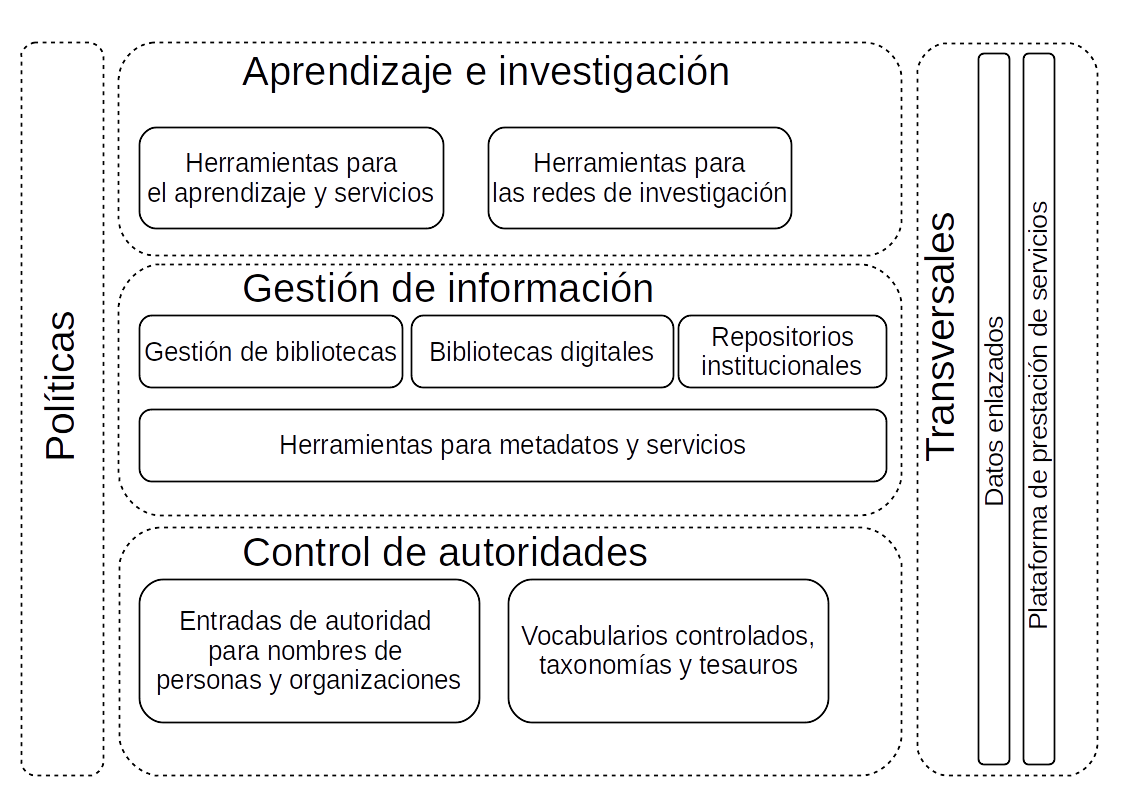
\includegraphics[width=0.5\textwidth]{img/referenceModel.png}
\end{center}
\caption{Modelo de referencia del proyecto ELINF. Fuente: Informe de autoevaluación de la primera fase del proyecto ELINF.}
\label{fig: referenceModel}
\end{figure}

En la redacción de artículos científicos se pueden encontrar variaciones de los nombres de un mismo autor, un autor puede tener varios nombres en artículos diferentes y varios autores pueden compartir el mismo nombre. Esta ambigüedad afecta el rendimiento de la recuperación de los documentos, la integración a nivel de bases de datos y puede causar atribuciones de autorías indebidas al aparecer los recursos descritos en los catálogos bajo un autor incorrecto \citep{Han2005}. En las bibliotecas, museos o en archivos un catálogo es un conjunto de datos organizados que describen los recursos de información gestionados por la institución \citep{InternationalFederationofLibraryAssociationsandInstitutions2009}, mientras que las personas encargadas de formar estos catálogos se denominan catalogadores \citep{RealAcademiaEspanola2014}. Durante al menos siglo y medio los catalogadores han documentado sus decisiones acerca de cómo la forma autorizada del nombre de una persona debería ser representada en sus catálogos \citep{Tillett2009}, sin embargo, según \cite{Carrasco2016} algunos tipos de inconsistencias que se encuentran a menudo en los nombres registrados en los catálogos son:

\begin{itemize}
\item Variantes del mismo nombre.
\item Permutaciones del nombre.
\item Errores tipográficos.
\item Eliminación de palabras vacías.
\item Eliminación de diacríticos.
\end{itemize}

Con la finalidad de evitar inconsistencias en los catálogos se realiza el control de autoridades, el cual es uno de los pilares del modelo de referencia del proyecto ELINF. El control de autoridades es el proceso de seleccionar una forma de un nombre y almacenarla, así como sus variantes y las fuentes de datos utilizadas en el proceso \citep{Sandberg2016}. Según \cite{Carrasco2016} este procedimiento sirve para dos propósitos fundamentales:

\begin{itemize}
\item Distinguir creadores que han publicado bajo el mismo nombre por medio de la adición de títulos y otras palabras asociadas con el nombre o incluyendo información sobre las fechas de nacimiento, muerte y actividad del mismo.
\item Identificar variantes del nombre o formas alternativas de escribirlo.
\end{itemize}

En el trabajo de las bibliotecas se ha estado lidiando con la identificación y desambiguación de los nombres de los creadores de los recursos de información desde los comienzos de la catalogación \citep{Harper2007}. Las diferentes formas utilizadas por el mismo creador en varias publicaciones y otros tipos de recursos siempre han acarreado cierto nivel de dificultad para agrupar sus creaciones \citep{Harper2007}.

Los catalogadores han creado registros para el control de autoridades durante décadas, resultando en grandes bases de datos con millones de registros como el ``Fichero de Nombres de Autoridades de la Biblioteca del Congreso'' (``Library of Congress Name Authority File'' - LC/NAF, por sus siglas de acuerdo al término en idioma inglés) \citep{Sandberg2016}.

Los ``Requerimientos Funcionales para Datos de Autoridad'' (``Functional Requirements for Authority Data'' – FRAD, por sus siglas de acuerdo al término en idioma inglés), elaborados en 2008 por la ``Federación Internacional de Asociaciones Bibliotecarias e Instituciones'' (``International Federation of Library Associations'' - IFLA, por sus siglas de acuerdo al término en idioma inglés), son un modelo entidad-relación enfocado en los datos de autoridad. Los FRAD enmarcan el control de autoridades en términos de entidades y relaciones entre personas y sus nombres; personas y sus obras, manifestaciones, expresiones y elementos \citep{InternationalFederationofLibraryAssociationsandInstitutions2009,Sandberg2016}.

El modelo que proponen los FRAD ha sido adoptado por las normas denominadas ``Recurso, Descripción y Acceso'' (``Resource, Description and Access''- RDA, por sus siglas de acuerdo al término en idioma inglés), que constituyen el código actual de control de autoridades \citep{Sandberg2016}.

Iniciativas existentes en la Web contribuyen a proveer mejores mecanismos para identificar a las personas que tienen un rol con respecto a recursos de información \citep{Harper2007}. ``Amigo de un amigo'' (``Friend of a friend'' - FOAF, por sus siglas de acuerdo al término en idioma inglés) es un proyecto que pretende crear una Web de páginas legibles por computadoras describiendo personas, sus vínculos y las cosas que crean y hacen. Encontrar formas de integrar este tipo de iniciativas con los mecanismos existentes en las bibliotecas para el control de autoridades puede contribuir a la inclusión de los catálogos bibliotecarios entre las herramientas disponibles en la Web. Adicionalmente, la disponibilidad de datos bibliotecarios de autoridad en formatos cada vez más compatibles con la Web, tiene el potencial para influenciar de manera positiva la organización de un amplio espectro de contenido disponible en la Web hoy día \citep{Harper2007}.

El ``Fichero Internacional Virtual de Autoridades'' (``Virtual International Authority File'' - VIAF, por sus siglas de acuerdo al término en idioma inglés) combina varios ficheros de nombres de autoridades en un solo servicio de nombres de autoridad. Para lograr esto, VIAF vincula los ficheros de autoridades de varias bibliotecas nacionales y agrupa todos los registros de autoridad para una entidad determinada en un ``súper registro de autoridad'' que unifica los diferentes nombres de dicha entidad \citep{OCLCOnlineComputerLibraryCenterInc.2014}.

Otra iniciativa ejecutada con el fin de contribuir al control de autoridades es el ``Identificador Internacional Estandarizado de Nombres'' (``International Standard Name Identifier'' - ISNI, por sus siglas de acuerdo al término en idioma inglés). ISNI es el número estándar global certificado para identificar a los contribuidores de trabajos creativos y a aquellos involucrados en su distribución como investigadores, inventores, escritores, artistas, creadores visuales, actores, productores entre otros \citep{ISNIInternationalStandardNameIdentifier2017}.

La misión de la Autoridad Internacional del ISNI (``ISNI International Authority'' - ISNI-IA, por sus siglas de acuerdo al término en idioma inglés) es asignarles a los nombres públicos de autores de recursos de información un número identificativo persistente con el objetivo de resolver el problema de la ambigüedad en la búsqueda y recuperación de la información respectiva a nombres de creadores de recursos de información \citep{ISNIInternationalStandardNameIdentifier2017}. Similares a esta iniciativa son las formas utilizadas por el Identificador Abierto de Investigador y Colaborador (``Open Researcher and Contributor ID'' - ORCID, por sus siglas de acuerdo al término en idioma inglés) \citep{ORCID2017} y el identificador de SCOPUS \citep{Elsevier2016}.

Con el objetivo de almacenar los datos con vistas a su posterior procesamiento y recuperación, variadas son las estructuras empleadas para realizar de forma eficiente esta tarea \citep{Gutierrez2011,Vavliakis2013,Lacasta2013}. Las bases de datos relacionales han sido empleadas durante varias décadas para estructurar los datos y recuperarlos de forma eficiente \citep{maier1983theory,Shanmugasundaram1999,Ilyas2004,Spanos2012}. En los últimos años la utilización de bases de datos ``No-SQL'' ha ganado popularidad con el objetivo de almacenar datos en forma de documentos \citep{Pokorny2013,Moniruzzaman2013}. La utilización del modelo de datos ``Marco de trabajo para la descripción de recursos'' (``Resource Description Framework'' - RDF, por sus siglas de acuerdo al término en idioma inglés) ha contribuido a aportar semántica a los datos almacenados, proveyendo un valor añadido a la información \citep{Berners-Lee2001,Konstantinou2014,Sule2016}.

En Cuba en el momento en que se realiza la presente investigación no existe un registro central para el control de autoridades, las instituciones realizan este proceso de forma aislada, provocando redundancia en el trabajo. De igual manera, no se reutilizan los registros de autoridades que comparten instituciones extranjeras. Esta situación dificulta la localización de la producción intelectual generada y/o almacenada en la Isla, a la vez que dificulta compartir las entradas de autoridad pertenecientes a autores cubanos con el resto del mundo.

La integración de fuentes de datos es el problema de interconectar y acceder a fuentes heterogéneas de datos \citep{Nachouki2011}. En la medida en que las organizaciones han evolucionado este problema se ha convertido en un importante campo de investigación tanto para la academia como para la industria \citep{Nachouki2011}. Aunque la dependencia conceptual es casi universal en el diseño de sistemas de información, también produce una gama de consecuencias negativas incluyendo la inflexibilidad de los sistemas, la heterogenidad en las formas de almacenar los datos, así como aumentos en los costos de mantenimiento \citep{McGinnes2015}. La heterogeneidad entre dos o más sistemas de bases de datos ocurre cuando estas utilizan diferente infraestructura de software o hardware, siguen diferentes convenciones sintácticas y modelos de representación o cuando interpretan de manera diferente datos similares \citep{Spanos2012}.

Con el propósito de contribuir a la solución de este problema en el pasado se propuso la creación de una base de datos federada (``Federated database'' - FDB, por sus siglas de acuerdo al término en idioma inglés) \citep{Sheth1990}. En arquitecturas de integración de bases de datos típicas, uno o más modelos conceptuales se utilizan para describir los contenidos de cada fuente de datos, las consultas se plantean en concordancia con un esquema conceptual global y para cada fuente de datos, una envoltura (``wrapper'', término utilizado en idioma inglés) es responsable de re-formular la consulta y recuperar los datos apropiados \citep{Spanos2012,Franke2014,ElKadiri2015}.

Un enfoque para la integración de datos empresariales provenientes de fuentes heterogéneas de datos y descentralizadas es la mediación semántica. Este enfoque por una parte elimina la necesidad de un repositorio central de datos o un esquema federado para todos los datos y, por otra parte, introduce una capa semántica encima de las descripciones de estructuras de datos sintácticas existentes para evitar los conflictos semánticos en la integración \citep{ElKadiri2015}. 

Con el advenimiento de la Web, la gestión de datos se enfocó en la variedad de información disponible en este nuevo medio. \cite{Janev2011} plantean que las tecnologías semánticas se utilizan en su mayoría para la integración de datos y para mejorar las búsquedas. Según \citep{Hoang2014}, la integración de datos guiada por ontologías representa una solución flexible, sostenible y extensible. Un paradigma reciente que combina la posibilidad de utilizar razonamiento sobre el conocimiento de un dominio codificado en una ontología, con un mecanismo que permite el uso de la misma ontología para un acceso integrado de alto nivel a las fuentes de datos es el Acceso e Integración de Datos Basado en Ontologías (``Ontology-Based Data Access and Integration'' - OBDA/OBDI, por sus siglas de acuerdo al término en idioma inglés) \citep{Calvanese2016,Calvanese2017}.

Teniendo en cuenta la heterogeneidad estructural de las fuentes de datos disponibles actualmente para realizar el control de autoridades en el proyecto ELINF se establece como \textbf{problema de investigación} el siguiente: ¿Cómo integrar los datos relativos al control de autoridades almacenados de forma heterogénea en las fuentes de datos utilizadas por el proyecto ELINF?

El problema de investigación se enmarca en el \textbf{objeto de estudio} la integración de datos almacenados de forma heterogénea y como \textbf{campo de acción} el método para integrar datos relativos al control de autoridades en el proyecto ELINF.

Esta investigación se propone como \textbf{objetivo general} desarrollar un método con componentes semánticos que permita la integración en una aplicación informática de datos relativos al control de autoridades, almacenados de forma heterogénea en las fuentes de datos utilizadas por el proyecto ELINF. Como \textbf{objetivos específicos} se definen los siguientes:

\begin{enumerate}
\item Identificar los referentes teóricos que soportan la integración semántica de datos en aplicaciones informáticas.
\item Desarrollar un método con componentes semánticos que permita integrar en una aplicación informática datos almacenados de forma heterogénea.
\item Evaluar el método desarrollado mediante un caso de estudio con datos reales relativos al control de autoridades almacenados de forma heterogénea.
\end{enumerate}

Se plantea como \textbf{hipótesis de la investigación} que, si se desarrolla un método con componentes semánticos para la integración de datos almacenados de forma heterogénea, será posible integrar los datos relativos al control de autoridades almacenados en las fuentes de datos utilizadas por el proyecto ELINF.

A partir de la hipótesis se identifica como variable independiente el \textbf{método con componentes semánticos} el cual se define como el conjunto de actividades \citep{Offermann2010} que permitirá conducir el proceso de descripción e integración de datos almacenados de forma heterogénea. Como variable dependiente se identifica la \textbf{integración de los datos relativos al control de autoridades} almacenados en las fuentes de datos utilizadas por el proyecto ELINF, definiéndose esta como la capacidad de mostrar en una vista conceptualmente homogénea datos de autoridades almacenados en fuentes heterogéneas de datos.


\begin{table}
\centering
\begin{tabular}{c|c|c}
\hline 
Variable & Dimensión & Indicadores \\ 
\hline 
Método con componentes semánticos & Etapas que lo componen & Artefactos generados \\ 
\hline 
Integración de los datos  & Fuentes integradas & Estructura de la fuente \\
relativos al control de autoridades & &  \\ 
 \hline
\end{tabular} 
\label{tabla:operacionalizacion}
\caption{Operacionalización de las variables de la investigación}
\end{table}


Durante toda la investigación se utilizará el método analítico - sintético, el mismo permitirá descomponer las problemáticas que se presenten en sus componentes y relaciones. La síntesis permitirá descubrir las relaciones esenciales existentes entre los componentes de las problemáticas contribuyendo a la sistematización del conocimiento. 

El método inductivo - deductivo posee especial relevancia en la formulación de la hipótesis y en la elaboración de conclusiones lógicas. Por medio del método histórico - lógico será posible representar los elementos del estado del arte relevantes a la temática en un orden cronológico que permita comprender la evolución de la misma.

El método hipotético - deductivo de conjunto con el inductivo - deductivo permitirá arribar a conclusiones particulares a partir de la hipótesis, que luego serán validadas experimentalmente. Esto posibilitará reafirmar la validez de la hipótesis de la investigación.

Por medio de la modelación será posible generar componentes relevantes para la aplicación del método propuesto, estando estrechamente relacionado con el método analítico - sintético y el método sistémico.

El documento de tesis está estructurado en tres capítulos, conclusiones y recomendaciones. A continuación, se brinda una breve descripción de cada uno de los capítulos.

El capítulo 1 aborda los principales referentes teóricos que soportan la integración semántica de datos, en él se refiere la evolución histórica del control de autoridades, se exponen los principales elementos de la Web Semántica y se relatan elementos de la integración de datos que son tomados en consideración para el desarrollo de la investigación.

En el capítulo 2 se identifica el paradigma utilizado en el desarrollo del método propuesto, se realiza la definición del método OntoIntegra a la vez que se describen cada uno de sus componentes. Se detalla el proceso de desarrollo de la ontología creada según la metodología seleccionada, generando cada uno de los artefactos definidos.

El capítulo 3 relata la selección de la estrategia de evaluación, la preparación del caso de estudio, su diseño con cada una de las etapas que lo componen. Se realiza un análisis de los datos recolectados que permite comprobar la validez de la hipótesis formulada para conducir la investigación.